% !TEX encoding = UTF-8 Unicode

\documentclass[a4paper]{article}


\usepackage{color}
\usepackage{url}
\usepackage{amsthm}
\usepackage[T2A]{fontenc} % enable Cyrillic fonts
\usepackage[utf8]{inputenc} % make weird characters work
\usepackage{graphicx}
\usepackage{subcaption}
\usepackage{amsmath}
\usepackage{verbatim}
\graphicspath{ {./images/} }

\usepackage[english,serbian]{babel}

\usepackage[unicode]{hyperref}
\hypersetup{colorlinks,citecolor=green,filecolor=green,linkcolor=blue,urlcolor=blue}

\newtheorem*{tvrdjenje}{Tvrđenje}
\newtheorem*{hipoteza}{Hipoteza}
\theoremstyle{definition}
\newtheorem{primer}{Primer}[section]



\begin{document}

\title{YouTube Trending\\ \small{Seminarski rad u okviru kursa\\Istraživanje podataka\\ Matematički fakultet}}

\author{Nikola Dimitrijević \footnote{mi14079@alas.matf.bg.ac.rs}\\
        Luka Živanović \footnote{mi14164@alas.matf.bg.ac.rs}\\
 }
%\date{9.~april 2015.}
\vspace*{-3cm}
    {\let\newpage\relax\maketitle}

\tableofcontents

\newpage



% ==============================================================================
\section{Uvod}
\label{sec:uvod}
% ==============================================================================

Skup podataka ``Trending YouTube Video Statistics'' sadrži informacije o YouTube video klipovima koji su se pojavili na Trending listi.
Klipovi koji se nalaze na Trendingu su u tom trenutku aktuelni, popularni ili relevantni. Neće svaki klip sa mnogo pregleda biti na trendingu,
 pritom se trending liste razlikuju za svaku državu. Podaci su nastali višemesečnim prikupljanjem klipova sa trending liste korišćenjem YouTube API.
Skup podataka se može naći na adresi \url{https://www.kaggle.com/datasnaek/youtube-new}.

% ==============================================================================
\section{Analiza i pretprocesiranje podataka}


\label{sec:analiza}
% ==============================================================================

\subsection{Opis skupa podataka}
Podaci se nalaze u više tabela: US, GB, DE,
CA i FR (SAD, Velika Britanija, Nemačka, Kanada i Francuska redom). 
Svaki klip se može naći više puta na trendingu.
Primera radi, US tabela sadrži 38549 redova, među kojima je zapravo  6201 različitih klipova.


\begin{table}[h!]
\centering
\begin{tabular}{ |c|c| } 
 \hline
 video\_id & jedinstveni identifikator svakog video klipa  \\ 
\hline
 trending\_date & datum kad je klip bio na trendingu (yy.dd.mm)  \\ 
\hline
 title & naziv klipa  \\ 
\hline
 channel\_title & naziv kanala koji je postavio klip  \\ 
\hline
 category\_id & jedinstveni identifikator tematske kategorije klipa  \\ 
\hline
publish\_time & vreme postavljanja klipa (yyyy-mm-ddThh:mm:ss.000Z)\\ 
\hline
tags & ključne reči, u formatu tag1|tag2|... |tagn  \\ 
\hline
views & broj pregleda  \\ 
\hline
likes & broj ljudi koji su izabrali da im se sviđa klip\\ 
\hline
dislikes & broj ljudi koji su izabrali da im se ne sviđa klip   \\ 
\hline
comment\_count & broj komentara \\ 
\hline
thumbnail\_link & link ka sličici koja predstavlja video klip  \\ 
\hline
comments\_disabled & da li su komentari isključeni  \\ 
\hline
ratings\_disabled & da li je ocenjivanje isključeno \\ 
\hline
video\_error\_or\_removed & da li video ima grešku ili je uklonjen  \\ 
\hline
description & opis video klipa  \\ 
 \hline
\end{tabular}
\caption{Opis datoteke USvideos.csv. Nazivi kolona su dati levo, a njihovi opisi desno.}
\label{table:1}
\end{table}

Ovaj skup podataka takođe sadrži i JSON datoteke za svaku od navedenih država.
Razlog za to je što se skup tematskih kategorija klipova razlikovao među državama, pa se u JSON datotekama nalaze imena koja odgovaraju određenim identifikatorima kategorija.

\subsection{Pretprocesiranje}

\begin{figure}[h!]
\begin{center}
    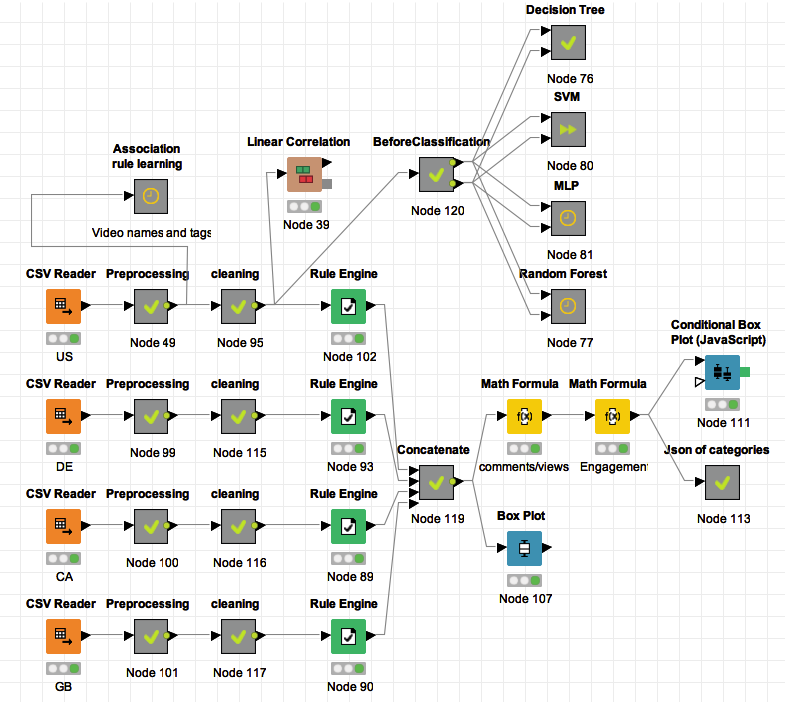
\includegraphics[width=1\textwidth]{Global.png}
    \caption{Globalni pogled na KNIME projekat}
\end{center}
\end{figure}

U donjem levom delu se učitavaju podaci iz .csv datoteka, pretprocesiraju, prečišćavaju, dodaje se redovima oznaka na koju državu se odnose.
Nakon toga se svi spajaju u jednu ogrmonu tabelu.

Preprocessing meta-čvor sadrži obrade koje su potrebne za sav dalji tok analize.


\begin{figure}[h!]
\begin{center}
    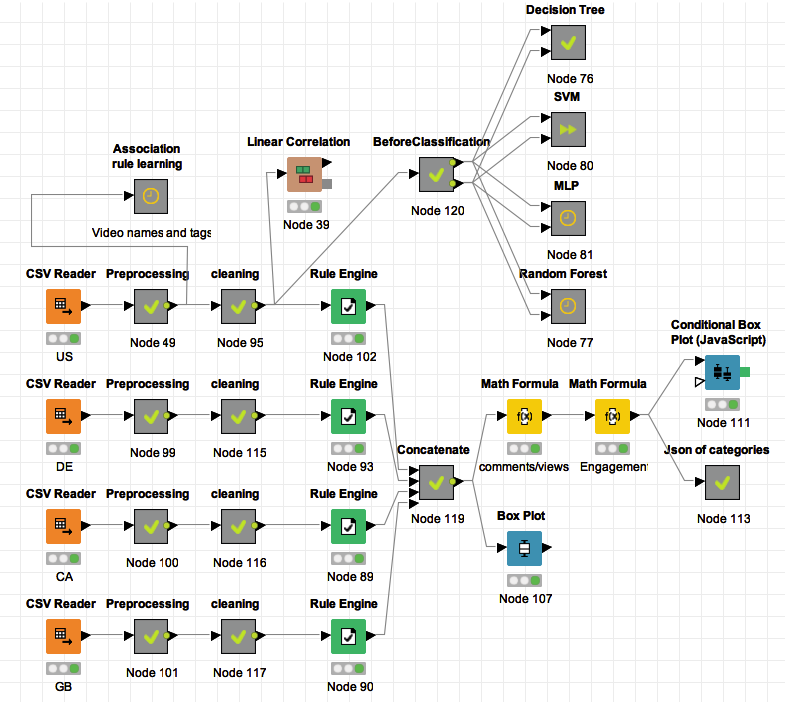
\includegraphics[width=1\textwidth]{Global.png}
    \caption{Pretprocesiranje}
\end{center}
\end{figure}
% ==============================================================================
\section{Klasifikacija}
\label{sec:klasifikacija}
% ==============================================================================
....
% ==============================================================================
\section{Pravila pridruživanja}
\label{sec:pravila}
% ==============================================================================

x <= {y, z}

% ==============================================================================
\section{One vizualizacije mozda ovde?}
\label{sec:dod}
% ==============================================================================


